\subsubsection{Digitaler Datenfluss}
\label{sec:Dataflow}

Anhand der nachfolgenden Abbildung \ref{pic:DMA_Dataflow} wird gezeigt, wie der Datenfluss durch den STM32 mit den jeweils verwendeten Datentypen, den Routinen und den Quelldateien aufgebaut ist.

\begin{figure}[H]
	\centering
	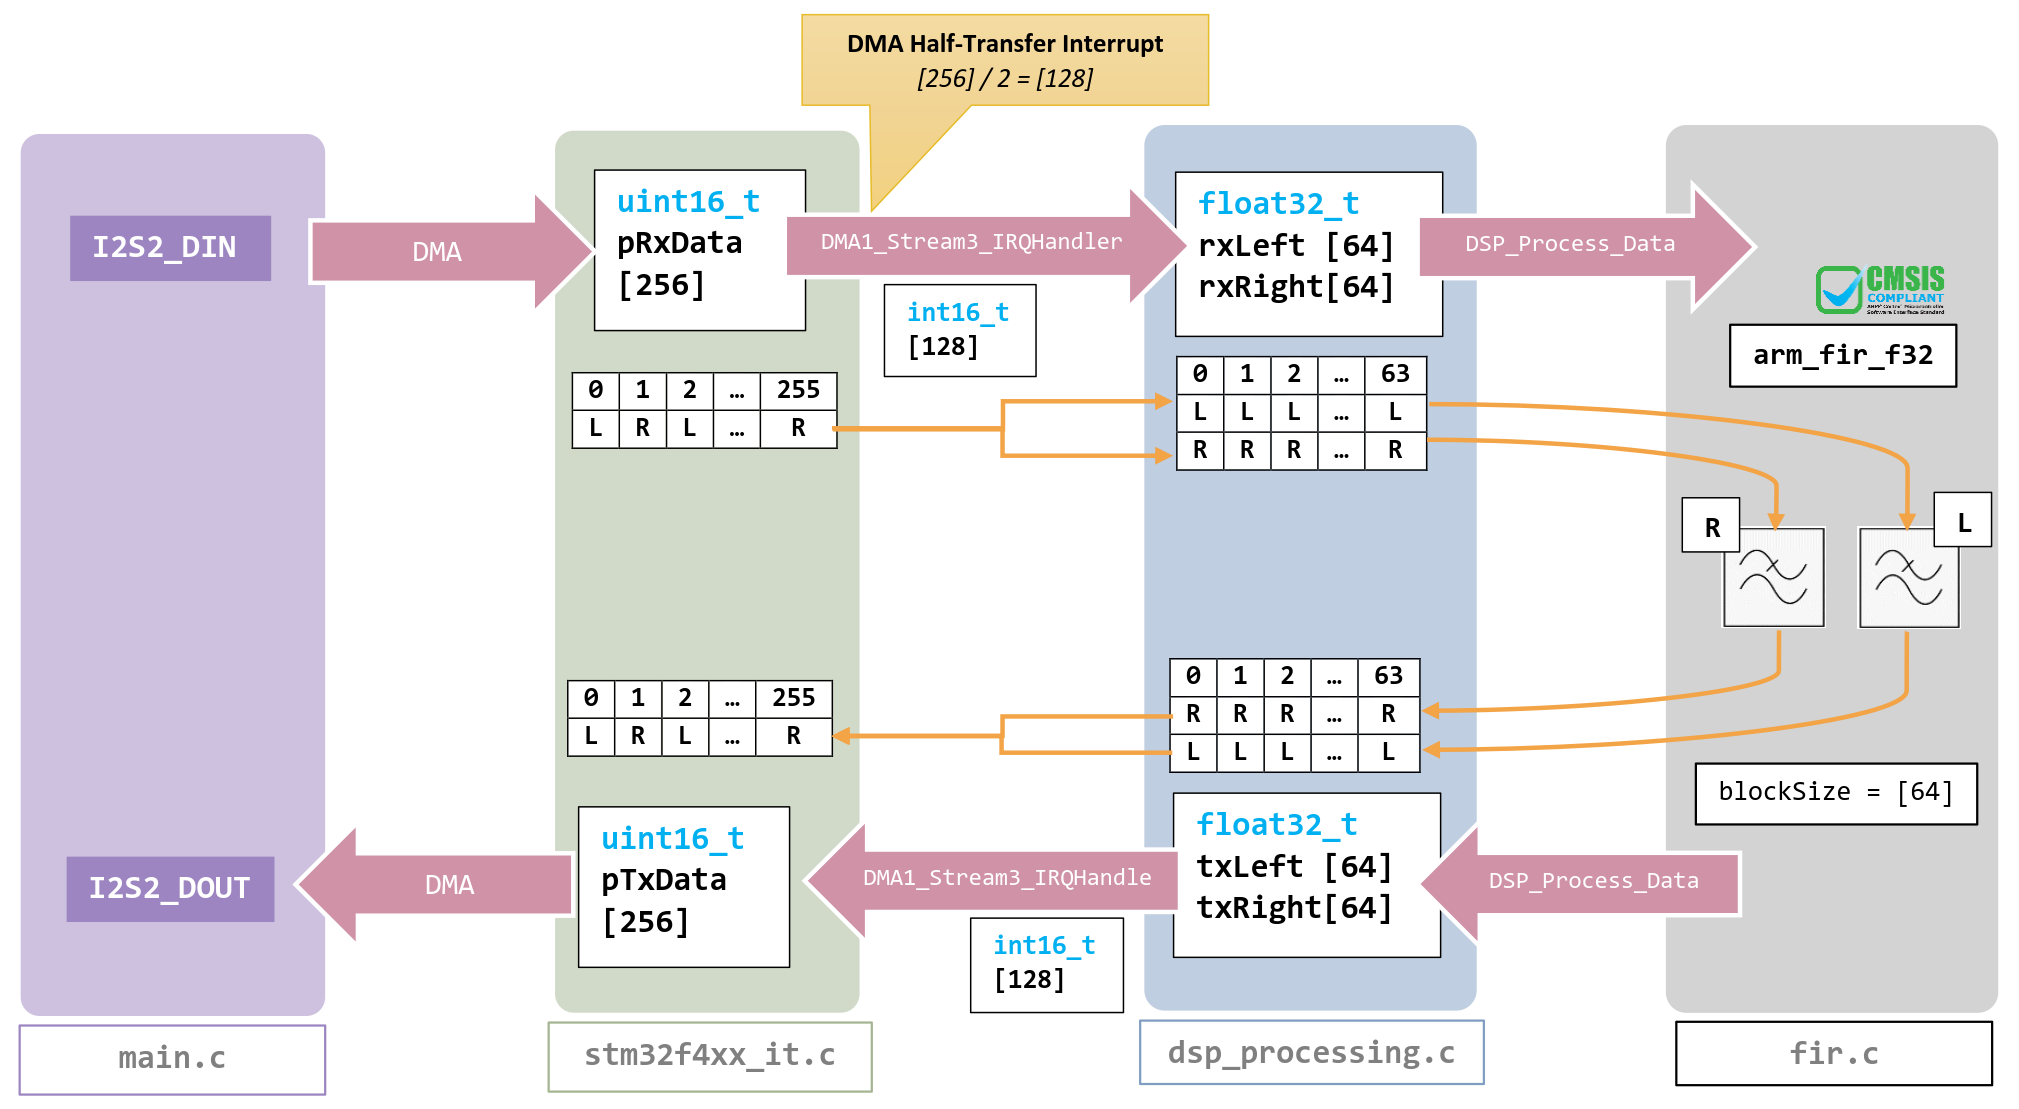
\includegraphics[width=1.0\linewidth]{DMA_Dataflow}
	\caption{Signalfluss des abgetasteten Audiosignals durch die verschiedenen Stufen der Verarbeitung}
	\label{pic:DMA_Dataflow}
\end{figure}


\paragraph{Ablauf der Datenverarbeitung}

Der DMA Controller wird im \texttt{main.c} so gestartet, dass ankommende Daten automatisch in den \texttt{uint16\_t} Buffer \texttt{pRxData} geschrieben werden. Die Datengrösse des DMA Buffers ist 256. 

Sobald der Buffer halb voll (128 Samples) ist, wird ein DMA Half-Transfer Interrupt ausgelöst.
Dieser Interrupt wird im der ISR \texttt{DMA1\_Stream3\_IRQHandler()} abgearbeitet. 
In der ISR werden die neuen gültigen Daten der Länge 128 an die Routine \texttt{DSP\_Process\_Data} übergeben, die die \texttt{uint16\_t} Werte explizit zu \texttt{int16\_t} castet. Ein Cast auf Signed ist notwendig, da das Audiosignal als signed zu interpretieren ist. Anschliessend folgt ein impliziter Cast auf \texttt{float32\_t}.

Bei der Wandlung auf \texttt{float32\_t} wird der Audiostream auf den linken und rechten Kanal in zwei Buffer \texttt{rxLeft} und \texttt{rxRight} aufgesplittet.
So stehen diese für die weitere Verarbeitung zur Verfügung durch verschiedene DSP Funktionen zur Verfügung.
Die beiden float-Buffer werden nun an die FIR Filterfunktion \texttt{FIR\_Filter\_F32\_Stereo} überreicht. In dieser Funktion wird ein zuvor initialisiertes FIR Filter aus der CMSIS/DSP Library ausgeführt.
Der Rückgabewert wird in den beiden Outputbuffern \texttt{txLeft} und \texttt{txRight} gespeichert.

Anschliessend folgt das Casting zurück zu \texttt{uint16\_t}. Bei diesem Schritt werden die Samples wieder auf die Anfangsreihenfolge mit abwechselnd linkem und rechtem Samplewert verteilt.
Der DMA Controller ist bereits im \texttt{main.c} so konfiguriert, diesen Outputbuffer \texttt{pTxData} automatisch über die \texttt{I2S2} Peripherie zu senden.

\begin{table}[H]
	\centering
	\begin{tabular}{|l|r|l|}
		\hline
		\textbf{\#define}       & \textbf{Wert} & \textbf{Beschreibung}                                                 \\ \hline
		\texttt{DSP\_BUFFERSIZE} & 128 & Anzahl Samples (L+R) pro DMA Interruptzyklus \\ \hline
		\texttt{DSP\_BUFFERSIZE\_HALF} & 64 & \begin{tabular}[c]{@{}l@{}}Anzahl Samples pro Kanal.\\ Auch blockSize für FIR Filter\end{tabular} \\ \hline
	\texttt{DSP\_BUFFERSIZE\_DOUBLE} & 256 & Grösse des Circular Buffers für den I2S DMA \\ \hline  
	\end{tabular}
	\caption{Erklärung der Werte im C-Code}
	\label{tab:buffer_sizes}
\end{table}

Die Tabelle \ref{tab:buffer_sizes} stellt den Bezug zu der Abbildung \ref{pic:DMA_Dataflow} und dem C-Code her. 

